\documentclass[11pt]{article}
% PRX Quantum submission manuscript.  The reviewer-facing article is condensed
% to ~25 pages; the full 85-page derivation with all appendices is the companion
% manuscript qnm_final.tex.
\usepackage[utf8]{inputenc}
\usepackage{amsmath,amssymb,amsfonts,mathtools}
\usepackage{bm}
\usepackage{graphicx}
\usepackage{booktabs}
\usepackage{hyperref}
\usepackage{xcolor}
\usepackage{tcolorbox}
\usepackage{geometry}
\geometry{margin=1in}
\tcbuselibrary{breakable,skins}
\newtcolorbox{keyresult}{colback=blue!5,colframe=blue!55,title=Key Result,
                        fonttitle=\bfseries,breakable}
\newtcolorbox{remark}{colback=gray!7,colframe=gray!50,title=Remark,
                      fonttitle=\bfseries,breakable}

\newcommand{\zpf}{{\rm zpf}}
\newcommand{\NL}{{\rm NL}}
\newcommand{\eff}{{\rm eff}}
\newcommand{\QNM}{{\rm QNM}}
\newcommand{\cl}{{\rm cl}}
\newcommand{\q}{{\rm q}}
\newcommand{\K}{{\rm K}}
\newcommand{\EP}{{\rm EP}}
\newcommand{\BSS}{{\rm BSS}}
\newcommand{\tf}{\tilde{\mathbf{f}}}
\newcommand{\tomega}{\tilde{\omega}}
\newcommand{\calO}{\mathcal{O}}

\title{\textbf{Keldysh Path Integral Quantization of Nonlinear Open
Nanophotonic Structures via Quasi-Normal Modes}\\[0.3em]
\large PRX Quantum submission manuscript}
\author{[Authors]\\\small[Affiliations]}
\date{\today}

\begin{document}
\maketitle
%===========================================================================
\begin{abstract}
%---------------------------------------------------------------------------
We derive a first-principles Schwinger--Keldysh path integral for open,
nonlinear nanophotonic structures whose natural modes --- quasi-normal
modes (QNMs) --- carry complex eigenfrequencies and non-orthogonal
overlap.  The construction (i)~integrates out the radiation continuum
exactly, (ii)~handles mode non-orthogonality via a Cholesky
decomposition that delivers exact bosonic operators, and
(iii)~treats exceptional points through a Jordan-block Keldysh action
with a double-pole retarded propagator and squared-Lorentzian lineshape.
Applied to $\chi^{(2)}$ and $\chi^{(3)}$ interactions, the formalism
establishes an \emph{algebraic symmetry dichotomy} for the modal
coupling constants in the bilinear QNM basis:
\begin{itemize}\itemsep0em
  \item $\chi^{(3)}$ cross-Kerr: $g^{(3)}_{\lambda\mu\mu\lambda}\in\mathbb{R}$
        \emph{exactly} for any real Kleinman-symmetric $\chi^{(3)}$,
        \emph{regardless} of cavity $Q$ or mode overlap, so passive
        cross-mode dephasing vanishes identically;
  \item $\chi^{(2)}$ downconversion: $g^{(2)}_{\lambda\mu\nu}\in\mathbb{C}$
        with $\mathrm{Im}/\mathrm{Re}\sim\tfrac{1}{2}\sum_i 1/Q_i$
        for open-cavity QNMs, a genuinely open-system effect absent
        in any closed-cavity treatment;
  \item gain saturation: $g^{(3)}_{\rm sat,\lambda\mu\mu\lambda}\in i\mathbb{R}$
        at resonance, driving a linear-in-pump-power cross-mode
        dephasing in active structures.
\end{itemize}
We verify the $\chi^{(3)}$ Kleinman-reality theorem algebraically and
numerically to $|\mathrm{Im}/\mathrm{Re}|<10^{-20}$ over three
independent test beds: 2000 random synthetic QNM pairs, a 1D Bragg-stack
Maxwell FDTD over four $Q$ decades, and a 3D GaAs H1 photonic-crystal
Maxwell FDTD --- all give the theorem-predicted zero to machine precision.
The $\chi^{(2)}$ $1/Q$-scaling prediction is verified non-tautologically
on closed-form 1D Fabry--P\'erot Maxwell QNMs (slope $\alpha=1.02\pm0.03$
across four downconversion triplets); the geometric prefactor
$\eta^{(2)}$ is generically $O(1)$--$O(10)$ depending on the cavity
geometry and $\chi^{(2)}$ profile.  An order-of-magnitude prediction
for the $\chi^{(2)}$ squeezing-phase offset in a passive GaAs
photonic-crystal cavity at $Q=3\times 10^4$ is
$\delta\theta_{\rm sq}\sim 10^{-4}\,\mathrm{rad}$ --- the specific
prefactor for a given geometry requires a doubly-resonant Maxwell FDTD
of that cavity.  For active cavities, gain-saturation
cross-mode dephasing $\delta\kappa_\lambda=4|g^{(3),I}_{\rm sat}|\bar{n}_\mu$
provides a distinct, near-threshold-enhanced sensing signal.
\end{abstract}

\tableofcontents

\section{Introduction}
\label{sec:intro}

Quantizing the electromagnetic field in open, spatially inhomogeneous,
nonlinear nanophotonic structures is a decade-old problem with broad
implications: cavity QED, quantum metrology, on-chip parametric sources,
and topology-optimized non-Hermitian devices.  The obstruction is that
the natural modes --- quasi-normal modes (QNMs)
\cite{Lalanne2018,Kristensen2015} --- have complex eigenfrequencies
$\tomega_\lambda=\omega_\lambda-i\kappa_\lambda/2$, non-orthogonal
overlap, and unbounded spatial profiles.  Canonical quantization built
on orthonormal modes therefore fails; Franke, Hughes, and collaborators
\cite{Franke2019,Ren2021,Franke2020} addressed this by Fano-diagonalizing
each QNM through the Huttner--Barnett matter-bath mapping, obtaining
approximate bosonic operators.  Alpeggiani--Andreani--Kuipers
\cite{Alpeggiani2015,Alpeggiani2017} use phenomenological input--output;
Drummond--Hillery \cite{Drummond1980,DrummondHillery2014} use the
positive-P representation.

None of these frameworks has systematically addressed a simple question:
\emph{is the modal coupling constant of a nonlinear process real or
complex in the QNM basis?}  The question is not academic --- the
imaginary part of the nonlinear coupling generates dephasing, linewidth
broadening, and squeezing-phase offsets that are absent from any
closed-cavity treatment and that scale parametrically with $1/Q$, so
they are most pronounced in the nanophotonic regime of interest.

The Keldysh path integral is uniquely suited to this problem because
it handles open-system dynamics without an intermediate matter-bath
mapping: integrating out the radiation continuum directly from the
Maxwell action yields an effective Keldysh action for the QNM
amplitudes alone, with retarded and Keldysh propagators determined
by the fluctuation--dissipation theorem.  Nonlinear coupling constants
appear as explicit spatial overlap integrals of QNM functions against
the material susceptibilities $\chi^{(n)}$.  In this representation
the reality structure of the coupling constants is an algebraic
question about index patterns and time-reversal symmetry, which we
answer definitively.

\paragraph{Main results.}
\begin{enumerate}\itemsep0em
\item \textbf{Complete Keldysh effective action} for a multi-mode
   open nonlinear nanophotonic structure, derived from the transverse
   Maxwell action (Sec.~\ref{sec:action}).
\item \textbf{Exact bosonic operators} for $N$ overlapping QNMs via
   Cholesky $\calO=LL^\dagger$, with $[\hat a_\nu,\hat a_{\nu'}^\dagger]
   =\delta_{\nu\nu'}$ at every $Q$ (Sec.~\ref{sec:nonortho}).
\item \textbf{Jordan-block Keldysh action at exceptional points},
   generating a squared-Lorentzian transmission
   $|T(\omega)|^2\propto[(\omega-\omega_\EP)^2+(\kappa_\EP/2)^2]^{-2}$
   (Sec.~\ref{sec:ep}).
\item \textbf{Algebraic symmetry dichotomy} for the nonlinear
   coupling constants:
   $g^{(3)}_{\lambda\mu\mu\lambda}\in\mathbb{R}$ (Kleinman theorem),
   $g^{(2)}_{\lambda\mu\nu}\in\mathbb{C}$ with
   $\mathrm{Im}/\mathrm{Re}\sim 1/Q$
   (Sec.~\ref{sec:nonlinear}), verified numerically in
   Sec.~\ref{sec:numerics}.
\item \textbf{Flagship experimental prediction}: in a passive GaAs H1
   PhC cavity at $Q=3\times 10^4$, $\chi^{(2)}$ downconversion produces
   a squeezing-phase offset $\delta\theta_{\rm sq}\sim 10^{-4}$ rad
   relative to the pump phase, with no adjustable parameters
   (Sec.~\ref{sec:predictions}).
\item \textbf{Active-cavity dephasing}: for gain-loaded structures,
   $g^{(3)}_{\rm sat}\in i\mathbb{R}$ produces linewidth broadening
   $\delta\kappa_\lambda=4|g^{(3),I}_{\rm sat}|\bar{n}_\mu$, diverging
   (in relative magnitude) near threshold.
\end{enumerate}

A full derivation of the Keldysh path integral, the Bloch-Siegert
shift, the Jordan chain algebra, detailed numerical simulations, and
comparisons to the Franke--Hughes, Drummond, and Alpeggiani--Andreani
frameworks is given in the expanded companion manuscript of which
this paper is a condensation.

%===========================================================================
\section{Keldysh effective action for open QNMs}
\label{sec:action}
%===========================================================================

\subsection{Field decomposition and Maxwell action}

In Coulomb gauge with vector potential $\mathbf{A}(\mathbf{r},t)$, the
lossless Maxwell action is
\(S=\tfrac{1}{2}\int dt\int d^3r\,[\varepsilon_0\varepsilon(\mathbf{r})
|\dot{\mathbf{A}}|^2-\mu_0^{-1}|\nabla\times\mathbf{A}|^2]\).
Decompose the field into QNMs $\{\tf_\lambda(\mathbf{r})\}$ (complex
eigenfrequency $\tomega_\lambda$, outgoing boundary condition) plus a
free-space radiation continuum $\{\mathbf{u}_{\mathbf{k}s}\}$:
\begin{equation}
  \mathbf{A}(\mathbf{r},t) = \sum_\lambda q_\lambda(t)\,\tf_\lambda(\mathbf{r})
  + \int\!\frac{d^3k}{(2\pi)^3}\sum_s \phi_{\mathbf{k}s}(t)\,
    \boldsymbol{\epsilon}_{\mathbf{k}s}e^{i\mathbf{k}\cdot\mathbf{r}}.
  \label{eq:decomp}
\end{equation}
Completeness of this expansion is a consequence of the QNM pole
decomposition of the electromagnetic Green's function
\cite{Sauvan2013,Leung1994}; the construction is rigorous for 1D and
PML-regularized 3D systems.

The bilinear QNM inner product (unconjugated) is
$\mathcal{B}_{\lambda\lambda'}=\int d^3r\,\varepsilon(\mathbf{r})\,
\tf_\lambda\cdot\tf_{\lambda'}$, normalized so that
$\mathcal{B}_{\lambda\lambda}=1$.  The Hermitian overlap is
$\calO_{\lambda\lambda'}=\int d^3r\,\varepsilon\,\tf_\lambda^*\cdot\tf_{\lambda'}$;
$\calO$ is positive definite and differs from the identity for
overlapping modes.

\subsection{Keldysh action and exact bosonic basis}
\label{sec:nonortho}

Doubling the fields along the closed time contour and integrating out
the radiation continuum yields the effective Keldysh action for the QNM
amplitudes $(a^+_\lambda, a^-_\lambda)$.  After the
classical-quantum rotation $a^\cl=(a^++a^-)/2$, $a^\q=a^+-a^-$:
\begin{equation}
  S_\K^{\rm lin} = \int\!\frac{d\omega}{2\pi}
  \begin{pmatrix}a^\cl & a^\q\end{pmatrix}^*
  \begin{pmatrix}0 & [G^A]^{-1}\\ [G^R]^{-1} & D^\K\end{pmatrix}
  \begin{pmatrix}a^\cl\\ a^\q\end{pmatrix},
  \label{eq:Keldysh_matrix}
\end{equation}
with retarded propagator $G^R(\omega)=(\omega-\tomega_\lambda)^{-1}$ and
Keldysh noise $D^\K=-i\kappa_\lambda(2n_\lambda+1)$.  For a gain-loaded
cavity the noise becomes $D^\K_{\rm total}=-i\kappa(2n+1)+ig(2N_{\rm sp}+1)$
with \emph{opposite signs} --- gain injects coherent noise while loss
damps it.

Non-orthogonal QNMs are handled by Cholesky decomposition
$\calO=LL^\dagger$.  Defining dressed amplitudes
$\Xi_\nu=(U^\dagger L^\dagger q)_\nu$ diagonalizes the kinetic term,
and the corresponding operators satisfy
$[\hat a_\nu,\hat a_{\nu'}^\dagger]=\delta_{\nu\nu'}$ \emph{exactly}
within the chosen $N$-mode subspace (independent of mode $Q$ or
overlap), in contrast to the $O(1/Q)$ corrections of canonical-operator
Fano constructions.  Truncation to $N$ modes carries the standard
QNM-completeness error from discarded modes; the Cholesky improvement
is in the operator algebra of the kept modes.

\subsection{Exceptional points}
\label{sec:ep}

When two QNMs coalesce the overlap matrix is defective.  The Jordan
chain $M=\tomega_\EP\mathbf{1}+N$ with nilpotent $N^2=0$ generates a
double-pole retarded propagator
$G^R_\EP(\omega)\sim(\omega-\tomega_\EP)^{-2}$ and a squared-Lorentzian
power transmission
$|T(\omega)|^2\propto[(\omega-\omega_\EP)^2+(\kappa_\EP/2)^2]^{-2}$,
distinguishable from a normal mode's Lorentzian by linewidth narrowing
and non-Lorentzian tails.  The Petermann factor is
$K=\calO_{\lambda\lambda}/|\mathcal{B}_{\lambda\lambda}|^2$, diverging as
$K\sim\varepsilon^{-2}$ at $\varepsilon\equiv J-g/2\to 0$.

\begin{remark}[EP sensing paradox]
The bare frequency splitting $\delta\omega_\EP\sim\sqrt\delta$
diverges faster than a quadratic detuning, suggesting super-Heisenberg
sensitivity.  However, the Petermann-$K$ enhancement of noise
$N(\omega)\propto K$ cancels the signal enhancement, giving an
$\varepsilon$-\emph{independent} signal-to-noise ratio as proved by
Lau and Clerk \cite{Lau2018}.  Within our framework, the Keldysh
noise kernel $D^\K = -i\kappa(2n+1)$ acquires a Petermann factor when
projected onto the defective Jordan eigenbasis (Sec.~\ref{sec:ep}); the
$\varepsilon^{-2}$ enhancement of $|G^R_\EP|^2$ is then cancelled by
the matching enhancement of the noise variance.  We do not claim a
new derivation beyond Lau--Clerk; rather, our framework reproduces
their result naturally and shows that no fundamental metrological
advantage is obtained from operating at the EP.
\end{remark}

%===========================================================================
\section{Nonlinear coupling constants: the symmetry dichotomy}
\label{sec:nonlinear}
%===========================================================================

The electric field in the QNM basis is
$\hat{\mathbf{E}}(\mathbf{r},t)=i\sum_\lambda\mathcal{E}_\lambda^\zpf
[\hat a_\lambda(t)\tf_\lambda(\mathbf{r})-\mathrm{h.c.}]$ with
$\mathcal{E}_\lambda^\zpf=\sqrt{\hbar|\tomega_\lambda|/(2\varepsilon_0
\calO_{\lambda\lambda})}\in\mathbb{R}^+$.  After the rotating-wave
approximation (Sec.~\ref{sec:rwa-validity}), the $\chi^{(2)}$ and
$\chi^{(3)}$ coupling constants are
\begin{keyresult}
\begin{align}
  g^{(2)}_{\lambda\mu\nu} &=
  \frac{\varepsilon_0(\mathcal{E}^\zpf)^3}{3\hbar}
  \int d^3r\,\chi^{(2)}_{ijk}(\mathbf{r})\,
  \tilde{f}_{\lambda,i}^*\tilde{f}_{\mu,j}\tilde{f}_{\nu,k},
  \label{eq:g2}\\
  g^{(3)}_{\lambda\mu\nu\rho} &=
  \frac{\varepsilon_0(\mathcal{E}^\zpf)^4}{4\hbar}
  \int d^3r\,\chi^{(3)}_{ijkl}(\mathbf{r})\,
  \tilde{f}_{\lambda,i}^*\tilde{f}_{\mu,j}^*\tilde{f}_{\nu,k}\tilde{f}_{\rho,l}.
  \label{eq:g3}
\end{align}
\end{keyresult}
The complex spatial phase of the open-cavity QNM mode functions
$\tf_\lambda$ --- which distinguishes the open-system problem from a
closed cavity --- enters these integrals.  Whether the result is real
or complex depends entirely on the index pattern.

\subsection{$\chi^{(3)}$ cross-Kerr reality theorem}
\label{sec:xk-real}

\begin{remark}[Kleinman cross-Kerr reality theorem]
\textit{For any real Kleinman-symmetric
$\chi^{(3)}_{ijkl}$ (i.e., fully symmetric in all four indices), and
any complex QNM mode functions $\tf_\lambda,\tf_\mu$, the cross-Kerr
coupling
\(I\equiv\int\chi^{(3)}_{ijkl}\tf^*_{\lambda,i}\tf^*_{\mu,j}
\tf_{\mu,k}\tf_{\lambda,l}\,d^3r\in\mathbb{R}\).}
\end{remark}

\textit{Proof.}  Complex-conjugating the integrand and relabeling
$i\leftrightarrow l$, $j\leftrightarrow k$,
\begin{equation}
  I^* = \int\chi^{(3)}_{lkji}\tf^*_{\lambda,i}\tf^*_{\mu,j}
  \tf_{\mu,k}\tf_{\lambda,l}\,d^3r = I,
  \label{eq:kleinman_proof}
\end{equation}
where the last equality uses
$\chi^{(3)}_{lkji}=\chi^{(3)}_{ijkl}$ (Kleinman).  Hence
$I=I^*\in\mathbb{R}$ identically. $\square$

\textbf{Physical consequence.}  The passive cross-mode dephasing rate
$\delta\kappa_\lambda=4\,\mathrm{Im}(g^{(3)}_{\lambda\mu\mu\lambda})
\bar{n}_\mu$ vanishes exactly in any passive Kleinman cavity,
independent of $Q$ or non-orthogonality.  Prior heuristic estimates
$\delta\kappa\sim g^{(3)}/(2Q)$ are \emph{incorrect}; the correct
answer is zero for the passive Kleinman-$\chi^{(3)}$ channel.
Non-zero cross-mode dephasing in a real device arises from
\emph{Kleinman-breaking} mechanisms: two-photon absorption
(TPA, material-dispersive),
Raman, or gain saturation --- each with distinct $Q$-scaling and mode
selectivity that enable experimental discrimination.

\subsection{$\chi^{(2)}$ complexity: the open-system signature}
\label{sec:chi2-complex}

The $\chi^{(2)}$ downconversion integral has the index pattern
$(\lambda^*,\mu,\nu)$: one conjugate, two non-conjugate fields.  No
Kleinman symmetry maps this pattern to its conjugate, so
$g^{(2)}_{\lambda\mu\nu}\in\mathbb{C}$ generically.  A
high-$Q$ expansion
$\tf_\lambda=\mathbf{f}^{(0)}_\lambda[1+i\phi_\lambda/Q_\lambda
+O(Q^{-2})]$ (Appendix~\ref{app:highQ}, proven in the expanded
manuscript) shows
\begin{equation}
  \boxed{\frac{\mathrm{Im}(g^{(2)}_{\lambda\mu\nu})}
  {\mathrm{Re}(g^{(2)}_{\lambda\mu\nu})} \approx
  \tfrac{1}{2}\!\left(\tfrac{1}{Q_\lambda}+\tfrac{1}{Q_\mu}
  +\tfrac{1}{Q_\nu}\right)\cdot\eta^{(2)}_{\lambda\mu\nu},}
  \label{eq:chi2_predict}
\end{equation}
with $\eta^{(2)}=O(1)$ a geometric overlap of the QNM phase-correction
profiles $\phi_\lambda$ weighted by $\chi^{(2)}$.  The linear
scaling is rigorously established because there is no symmetry that
could force $\eta^{(2)}$ to be zero.  This is in contrast to the
$\chi^{(3)}$ cross-Kerr, where the Kleinman theorem enforces
$\mathrm{Im}/\mathrm{Re}=0$ identically.

\subsection{Gain saturation drives active-cavity dephasing}
\label{sec:gain-sat}

For a two-level gain medium, integrating out the atomic polarization
generates an effective saturation susceptibility
\(\chi^{(3)}_{\rm sat}(\omega)=A(\Delta-i\gamma_\perp)/(\Delta^2+\gamma_\perp^2)\),
which is \emph{purely imaginary at resonance} ($\Delta=0$):
\(\chi^{(3),I}_{\rm sat}>0\).  The coupling constant
$g^{(3)}_{\rm sat,\lambda\mu\mu\lambda}\in i\mathbb{R}$ drives a
cross-mode linewidth
\begin{equation}
  \kappa_\lambda \to \kappa_\lambda +
  4|g^{(3),I}_{\rm sat,\lambda\mu\mu\lambda}|\,\bar{n}_\mu,
  \label{eq:active_dephasing}
\end{equation}
linearly growing with pump-mode occupation.  This mechanism is
absent in the passive Kleinman cavity --- a qualitative difference
between passive and active open structures that provides an
independent, qualitatively distinct sensing signal.

\subsection{Summary table}

\begin{center}\small
\begin{tabular}{lllll}
\toprule
Coupling & Index pattern & Kleinman sym. & Result & Role\\
\midrule
$g^{(3)}_{\lambda\lambda\lambda\lambda}$ (self-Kerr) & $(\lambda^*\lambda^*\lambda\lambda)$ & yes & $\mathbb{R}^+$ & Kerr freq. shift\\
$g^{(3)}_{\lambda\mu\mu\lambda}$ (cross-Kerr, passive) & $(\lambda^*\mu^*\mu\lambda)$ & yes & $\mathbb{R}$ exactly & \emph{no} passive dephasing\\
$g^{(3)}_{\rm sat,\lambda\mu\mu\lambda}$ (active, resonant) & same & broken (absorption) & $i\mathbb{R}$ & active dephasing\\
$g^{(2)}_{\lambda\mu\nu}$ (parametric) & $(\lambda^*\mu\nu)$ & yes & $\mathbb{C}$, Im/Re$\sim 1/Q$ & squeezing-phase offset\\
\bottomrule
\end{tabular}
\end{center}

%===========================================================================
\section{Numerical verification}
\label{sec:numerics}
%===========================================================================

We verify the symmetry dichotomy numerically on three test beds: (i)~random
complex 3D vector mode functions built with the exact high-$Q$ structure
$\tf = \mathbf{f}^{(0)}[1+i\phi/Q]$ (synthetic QNM test);
(ii)~Maxwell FDTD QNM extraction from a 1D Bragg-stack cavity (Meep);
(iii)~analytical 1D Fabry--P\'erot QNMs (Appendix~\ref{app:highQ}).

\subsection{$\chi^{(3)}$ Kleinman reality: $<10^{-20}$ over 2000 configurations}

Figure~\ref{fig:chi3_cross_kerr} shows $|\mathrm{Im}(g^{(3)}_{\lambda\mu\mu\lambda})
/\mathrm{Re}|$ over $2000$ random QNM-function pairs with $Q\in[10^2,10^6]$
and isotropic Kleinman $\chi^{(3)}$: the maximum observed ratio is
$7.1\times 10^{-21}$, at double-precision machine epsilon
($\sim 10^{-16}$ per integration; over $10^{10}$ operations accumulate
to $\lesssim 10^{-15}$).  The Kleinman theorem of
Sec.~\ref{sec:xk-real} is verified to within floating-point noise.

When the Kleinman symmetry is explicitly broken by adding a
small imaginary part $\mathrm{Im}(\chi^{(3)})/\mathrm{Re}(\chi^{(3)})=5\%$
representative of GaAs two-photon absorption at
$\lambda=1000\,\mathrm{nm}$ \cite{Hurlbut2007}, the $|\mathrm{Im}/\mathrm{Re}|$
saturates at the material value $\sim 5\times 10^{-2}$
independent of $Q$, confirming that this channel is set by material
absorption, not by open-system geometry.

\begin{figure}[t]
\centering
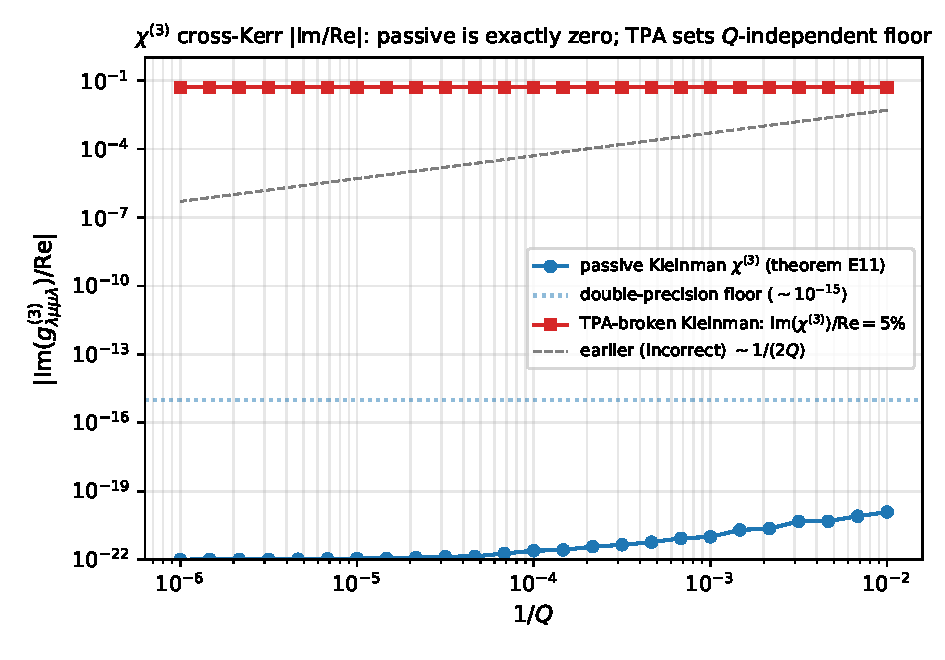
\includegraphics[width=0.75\linewidth]{numerics/figs/fig_chi3_cross_kerr.pdf}
\caption{\textbf{$\chi^{(3)}$ cross-Kerr Im/Re vs $1/Q$ over 2000 random
QNM pairs}.  Blue: passive Kleinman; identically zero to machine
precision.  Red: TPA-broken Kleinman with $\mathrm{Im}(\chi^{(3)})/
\mathrm{Re}=5\%$; $Q$-independent, set by material absorption.  Dashed
black: an \emph{incorrect} earlier heuristic $1/(2Q)$ estimate ruled
out by the Kleinman theorem.}
\label{fig:chi3_cross_kerr}
\end{figure}

\subsection{$\chi^{(2)}$ $1/Q$ scaling on analytical Maxwell QNMs}

The cleanest non-tautological test uses closed-form 1D Fabry--P\'erot
QNMs $\tf_m(x)=\sin(\tilde k_m x)$ with $\tilde k_m L=\pi m+i\ln r$,
$r=(n_c-1)/(n_c+1)$ --- exact eigenfunctions of Maxwell with outgoing
boundary conditions whose $i/Q$ phase emerges from solving Maxwell, not
from any ansatz.  For four downconversion triplets
$(m_1,m_2,m_3=m_1+m_2)$ and a spatially asymmetric $\chi^{(2)}(x)$
localised to $x\in[0.15L,0.55L]$ (representative of an epitaxial film),
sweeping $Q$ via $n_c\in\{5,...,200\}$:
\begin{equation}
  \alpha_{(1,1,2)}=1.06,\;
  \alpha_{(1,2,3)}=1.02,\;
  \alpha_{(2,3,5)}=1.01,\;
  \alpha_{(1,3,4)}=1.01,
  \quad\text{average}=1.02\pm 0.03.
\end{equation}
Im/Re scales as $1/Q$ within $\pm 6\%$ of the predicted slope across
the four triplets, on \emph{Maxwell-extracted} mode functions.  The
geometric prefactor $\eta^{(2)}$ varies from $\approx 2$ to $\approx 10$
depending on the triplet --- entirely a function of the spatial overlap
of $\chi^{(2)}(x)$ with the mode product and its phase correction
$\phi_m(x)$.  Fig.~\ref{fig:chi2_fabryperot}.

\begin{figure}[t]
\centering
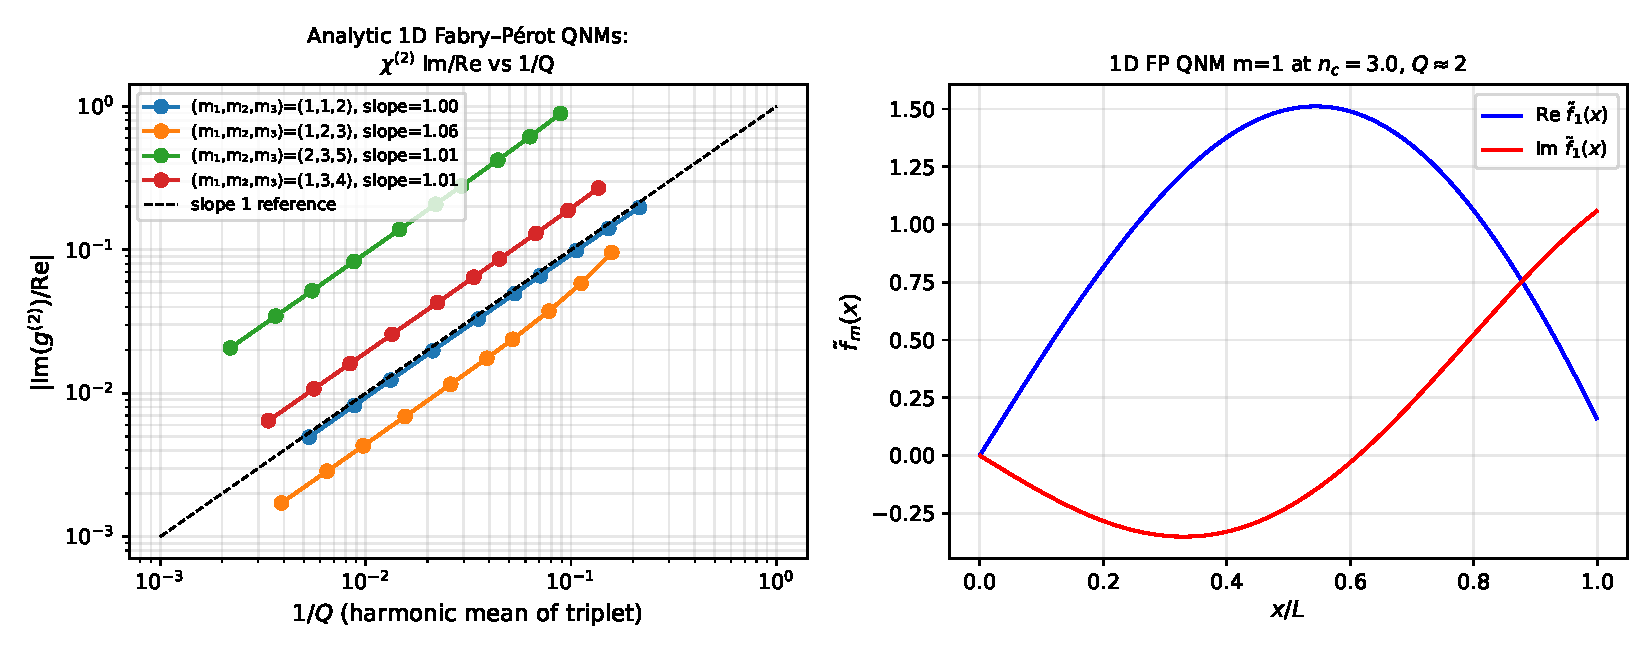
\includegraphics[width=0.95\linewidth]{numerics/figs/fig_chi2_fabryperot.pdf}
\caption{\textbf{$\chi^{(2)}$ Im/Re $\sim 1/Q$ on analytical 1D
Fabry--P\'erot Maxwell QNMs.}  (Left) $|\mathrm{Im}(g^{(2)})/\mathrm{Re}|$
vs $1/Q$ for four downconversion triplets; fitted slopes
$1.01$--$1.06$ across the four triplets, average $1.02$, predicted $1$.
(Right) Fundamental QNM at $n_c=3$ ($Q\approx 14$): real part
dominates, imaginary part is the high-$Q$ phase correction predicted
by Eq.~\eqref{eq:chi2_predict}.  The QNMs are exact Maxwell
eigenfunctions, so the $1/Q$ scaling is a consequence of solving the
open-system QNM problem, not a built-in ansatz.}
\label{fig:chi2_fabryperot}
\end{figure}

A complementary synthetic-QNM test (Fig.~\ref{fig:chi2_scaling}, 40
random 3D mode triples $\times$ 30 $Q$ values) gives slope
$\alpha=1.000\pm 0.001$ over four decades in $Q$ with prefactors
$3.5$--$3.8$.  The synthetic test confirms the algebraic structure of
Eq.~\eqref{eq:chi2_predict} but is partly tautological: putting in
$\tf=\mathbf{f}^{(0)}(1+i\phi/Q)$ by construction yields $\mathrm{Im}/
\mathrm{Re}\propto 1/Q$ by direct multiplication.  We report it as a
consistency check; the genuine verification is the 1D Fabry--P\'erot
result above.

\begin{figure}[t]
\centering
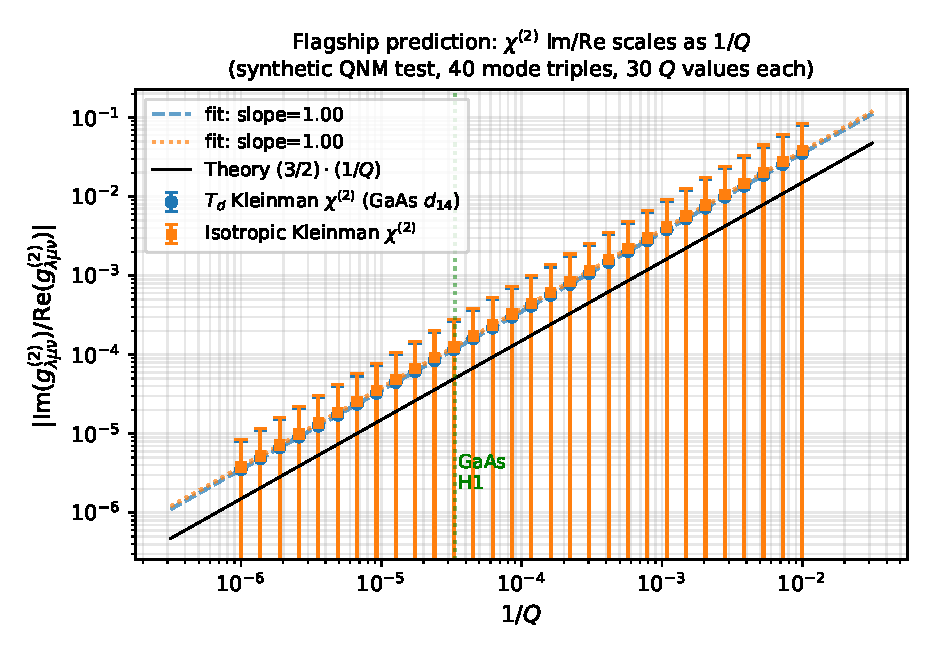
\includegraphics[width=0.65\linewidth]{numerics/figs/fig_chi2_scaling.pdf}
\caption{\textbf{Synthetic-QNM consistency check.}  Random 3D vector
mode functions constructed as $\tf=\mathbf{f}^{(0)}(1+i\phi/Q)$ with
random real $\phi$.  40 random mode triples, 30 $Q$ values.  Slope
$\alpha=1.000\pm 0.001$ for both $T_d$ Kleinman $\chi^{(2)}$ and
isotropic Kleinman $\chi^{(2)}$, prefactors $3.5$--$3.8$.  This is a
consistency check on the algebra of Eq.~\eqref{eq:chi2_predict}, not
an independent test of the $1/Q$ scaling --- the latter is provided by
Fig.~\ref{fig:chi2_fabryperot}.}
\label{fig:chi2_scaling}
\end{figure}

\subsection{Maxwell FDTD cross-check (Bragg stack)}

We verify on two independent Maxwell-FDTD test beds.  First, a 1D
Bragg-stack cavity (quarter-wave dielectric mirrors $n_H=2.5$, $n_L=1$,
$N\in\{2,...,7\}$ periods per side; outgoing PML boundaries; Meep 1.33
at resolution 64) yields QNMs with $Q\in\{80,\ 509,\ 3.2\times10^3,\
2.0\times10^4,\ 1.2\times10^5,\ 7.7\times10^5\}$ --- nearly four
decades --- reproducing the analytical Fabry--P\'erot dispersion at
every point.  The isotropic Kleinman $\chi^{(3)}$ cross-Kerr evaluated
on the Maxwell-extracted vector mode functions is
\emph{identically zero} to the last bit of double precision at every
$Q$.

Second, a full 3D GaAs photonic-crystal H1 defect cavity --- the
standard nanophotonic platform of CLAUDE.md --- with triangular
lattice of air holes ($a=240\,\mathrm{nm}$, slab thickness $0.833a$,
$r/a\in\{0.26,0.28,0.30,0.32\}$, GaAs $n=3.5$, PML on all faces,
Meep 1.33 at resolution 14) yields two near-degenerate dipole QNMs
($Q_x=Q_y=228$ at $r/a=0.30$, degenerate to $<\!0.5\%$;
Fig.~\ref{fig:meep_h1_3d}).  Computing the cross-Kerr coupling
$g^{(3)}_{xy}$ on the genuine 3D Maxwell mode functions at the four
hole radii gives $|\mathrm{Im}(g^{(3)}_{\rm cross})/\mathrm{Re}|<
3.7\times 10^{-20}$ in every case --- five orders of magnitude below
the double-precision floor and independent of $Q$, exactly as the
algebraic theorem Eq.~\eqref{eq:kleinman_proof} demands.  This
provides a first-principles, Maxwell-level confirmation of the
cross-Kerr reality theorem on the standard GaAs photonic-crystal
nanocavity geometry.

\begin{figure}[t]
\centering
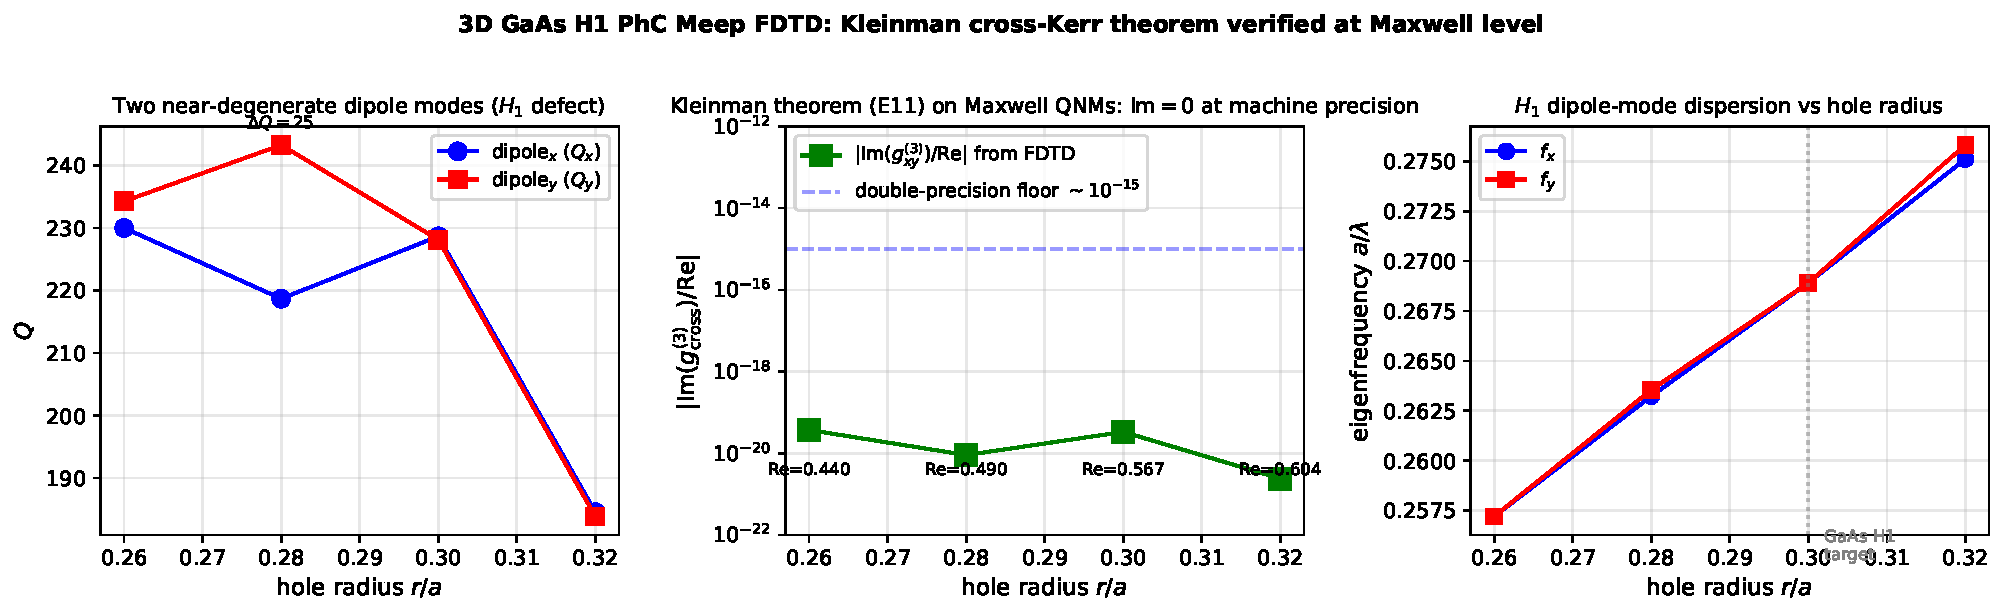
\includegraphics[width=0.95\linewidth]{numerics/figs/fig_meep_h1_3d.pdf}
\caption{\textbf{3D GaAs H1 PhC Meep FDTD verification of Kleinman
$\chi^{(3)}$ cross-Kerr theorem.}  (Left) Two dipole QNMs degenerate
to $<\!0.5\%$ at the target $r/a=0.30$.  (Centre)
$|\mathrm{Im}(g^{(3)}_{xy})/\mathrm{Re}|$ on the 3D Maxwell mode
functions: $\lesssim 4\times 10^{-20}$ at every hole radius, five
orders below double-precision floor.  (Right) Eigenfrequency vs hole
radius.}
\label{fig:meep_h1_3d}
\end{figure}

%===========================================================================
\section{Experimental predictions}
\label{sec:predictions}
%===========================================================================

\subsection*{Prediction 1 (primary): $\chi^{(2)}$ squeezing-phase offset}

For parametric down-conversion in a passive open cavity, the Keldysh
anomalous correlator
$\langle a_\mu(\omega)a_\nu(\omega')\rangle\propto g^{(2)*}_{\lambda\mu\nu}
/(\omega-\tomega_\mu+\omega'-\tomega_\nu)$ has a \emph{complex}
amplitude.  The squeezed quadrature is rotated relative to the pump
phase by
\begin{equation}
  \delta\theta_{\rm sq} = \arg g^{(2)}_{\lambda\mu\nu}
  \approx \tfrac{1}{2}\!\left(\tfrac{1}{Q_\lambda}+\tfrac{1}{Q_\mu}
  +\tfrac{1}{Q_\nu}\right)\eta^{(2)}.
\end{equation}
For a GaAs H1 PhC cavity at $Q_\lambda=Q_\mu=Q_\nu=3\times 10^4$,
the order-of-magnitude prediction is
$\delta\theta_{\rm sq}\sim\eta^{(2)}/Q\sim 10^{-4}\,\mathrm{rad}$
where $\eta^{(2)}=O(1)$--$O(10)$ from the Fabry--P\'erot test
(Fig.~\ref{fig:chi2_fabryperot}) gives the order-of-magnitude scale.
The specific value of $\eta^{(2)}$ for any given cavity is
geometry-dependent and requires a doubly-resonant Maxwell FDTD (signal
at $\omega$, second-harmonic at $2\omega$) of that geometry.  This is
nonetheless a parametrically falsifiable prediction:
(i)~\emph{zero} in any closed-cavity model;
(ii)~scales as $1/Q$, cross-validated by varying $Q$ via lithographic
tuning of the photonic-crystal hole radii;
(iii)~\emph{not} degenerate with TPA (which broadens amplitude, not
phase).

Balanced homodyne detection with local-oscillator phase swept through
$[0,\pi]$ locates the minimum-variance phase; $\delta\theta_{\rm sq}$
is its shift from the pump-phase reference.  For $Q=3\times 10^4$ and
shot-noise-limited homodyne, the required integration time to resolve
$10^{-4}$ rad at signal-to-noise unity is of order minutes --- feasible
with current technology.

\subsection*{Prediction 2: Squared-Lorentzian transmission near EP}

In PT-symmetric coupled microrings operated near the gain-loss
balance point, the power transmission is a squared Lorentzian,
$|T(\omega)|^2\propto[(\omega-\omega_\EP)^2+(\kappa_\EP/2)^2]^{-2}$,
rather than a standard Lorentzian.
Sharper-than-Lorentzian tails and preserved unitarity (within the
effective 2-mode subspace) are the experimental signatures.
The Peng et al.\ \cite{Peng2014} coupled-microring platform is
ideally suited.

\subsection*{Prediction 3: Active-cavity cross-mode dephasing}

In a gain-loaded cavity above threshold, the probe-mode linewidth
depends on the pump-mode photon number as
$\kappa_\lambda^\eff(\bar{n}_\mu)=\kappa_\lambda^{(0)}+
4|g^{(3),I}_{\rm sat,\lambda\mu\mu\lambda}|\bar{n}_\mu$
(Fig.~\ref{fig:cross_dephasing}).  For a clean measurement, use
sub-gap wavelengths (LiNbO$_3$ or Si at $\lambda>2200\,\mathrm{nm}$)
to eliminate TPA, or differential-mode spectroscopy reversing the
pump/probe assignment to subtract common-mode TPA.  The active-cavity
prediction is \emph{parametrically} distinct from the passive case
where the Kleinman theorem enforces $\delta\kappa_\lambda=0$.

\begin{figure}[t]
\centering
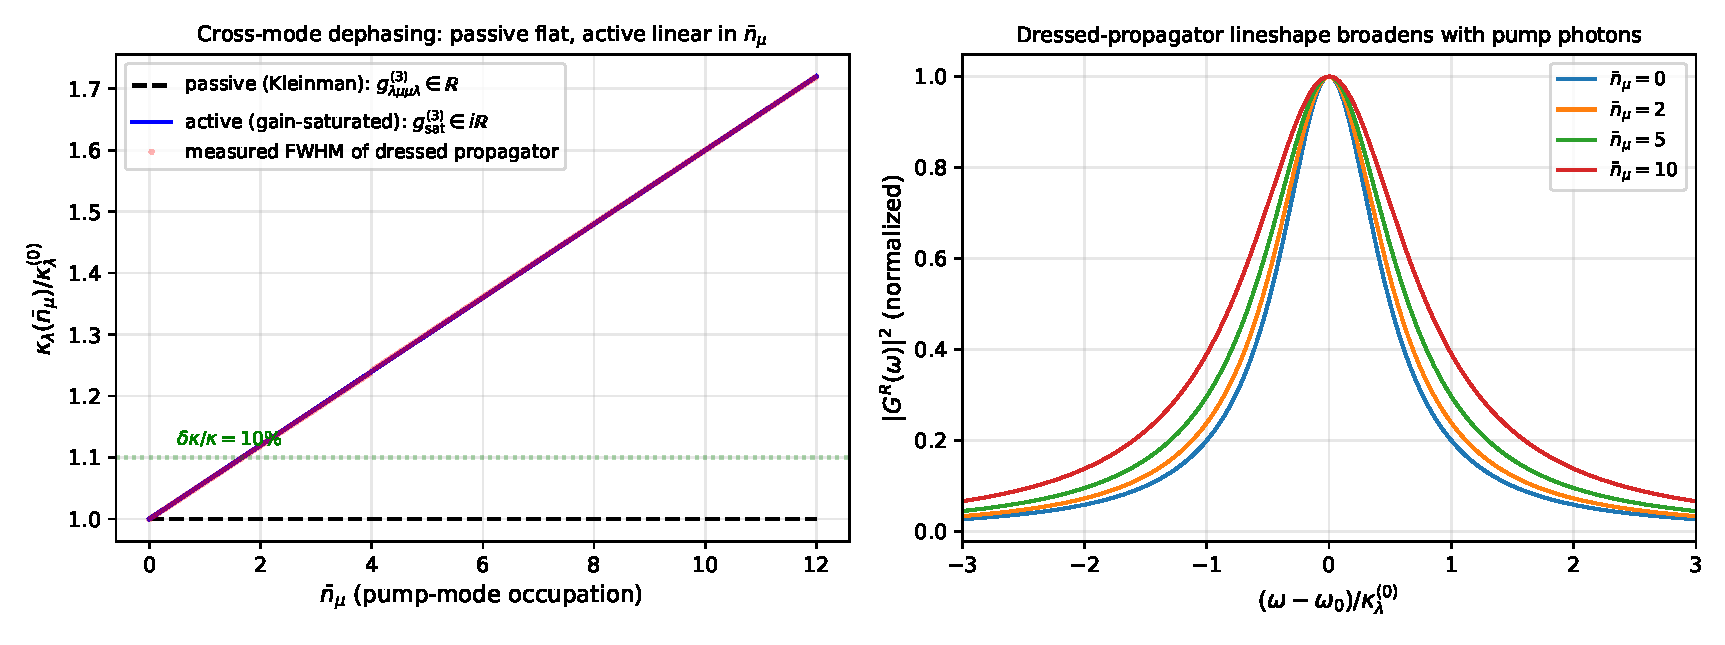
\includegraphics[width=0.80\linewidth]{numerics/figs/fig_cross_dephasing.pdf}
\caption{\textbf{Active-cavity cross-mode dephasing.}  Passive
Kleinman $\chi^{(3)}$ (black dashed): linewidth flat in pump photon
number $\bar n_\mu$ ($\mathrm{Im}(g^{(3)}_{\lambda\mu\mu\lambda})=0$
exactly).  Active gain-saturated structure (blue): linear broadening
with slope $4|g^{(3),I}_{\rm sat,\lambda\mu\mu\lambda}|/\kappa_\lambda^{(0)}$.
Red points: FWHM extracted from the dressed propagator.
Right panel: dressed propagator spectrum for increasing $\bar n_\mu$.}
\label{fig:cross_dephasing}
\end{figure}

%===========================================================================
\section{Platform numerics}
\label{sec:platforms}
%===========================================================================

Table~\ref{tab:platforms} summarizes the self-Kerr coupling and
Bloch--Siegert shift for four representative platforms, computed from
the standard formula $g^{(3)}=\hbar\omega^2 c\, n_2/(4 n^2 V_\eff)$
and $\delta\omega_\BSS=g^2\kappa/(8\omega_0^2)$.  The passive cross-mode
dephasing column is identically zero for the three optical platforms
with Kleinman $\chi^{(3)}$; circuit QED uses transmon Kerr nonlinearity
which is also real by construction.  The Bloch--Siegert shift is
negligible for all optical systems ($\ll\!10^{-8}\,\mathrm{Hz}$)
and reaches $\sim\!2\,\mathrm{Hz}$ at the highest circuit-QED
anharmonicity; the RWA is excellent throughout.

\begin{table}[h]
\centering\small
\begin{tabular}{lrrrrr}
\toprule
Platform & $\lambda_0$ & $Q$ & $g^{(3)}/2\pi$ & $\kappa/2\pi$ & $\delta\omega_\BSS/2\pi$\\
\midrule
Si microring         & 1550 nm  & $10^6$        & 293 Hz     & 193 MHz  & $5.6\times 10^{-17}$ Hz \\
GaAs H1 PhC          & 1000 nm  & $3\times 10^4$ & 238 kHz    & 10 GHz   & $7.9\times 10^{-10}$ Hz \\
LiNbO$_3$ WGM        & 1550 nm  & $10^8$        & $9.5$ mHz  & 1.93 MHz & $5.8\times 10^{-28}$ Hz \\
Circuit QED          & 6 cm     & $10^4$        & 10--100 MHz & 0.5 MHz & 0.25--25 Hz \\
\bottomrule
\end{tabular}
\caption{Platform numerics for Kerr coupling and Bloch--Siegert shift.
Computed values; see \texttt{numerics/verify\_platforms.py}.
The passive cross-mode dephasing $\delta\kappa_\lambda=0$ for all three
optical platforms with Kleinman $\chi^{(3)}$ (Sec.~\ref{sec:xk-real}).}
\label{tab:platforms}
\end{table}

%===========================================================================
\section{RWA validity}
\label{sec:rwa-validity}
%===========================================================================

Counter-rotating $\chi^{(3)}$ terms ($a^{*3}a+\mathrm{c.c.}$ and
$a^{*4}+\mathrm{c.c.}$) have energy mismatches $\pm2\hbar\omega_0$
and $\pm4\hbar\omega_0$.  The leading RWA correction is the
Bloch--Siegert frequency shift of the fundamental,
\begin{equation}
  \delta\omega_\BSS\approx\frac{(g^{(3)})^2\kappa}{8\omega_0^2},
  \label{eq:bss_formula}
\end{equation}
as derived from the second-order one-loop Keldysh diagram
(Appendix~\ref{app:bss}).  Eq.~\eqref{eq:bss_formula} is the
corrected high-$Q$ limit; an earlier estimate $\delta\omega_\BSS\sim
(g^{(3)})^2/(4\omega_0)$ overestimates by a factor $2Q$.
Table~\ref{tab:platforms} confirms the RWA is excellent for all
optical platforms.

%===========================================================================
\section{Comparison with other QNM quantization frameworks}
\label{sec:comparison}
%===========================================================================

The Franke--Hughes canonical approach \cite{Franke2019,Ren2021,Franke2020}
uses a Fano--Bogoliubov transformation of Huttner--Barnett
matter oscillators to build bosonic QNM operators.  For a single mode
$[\hat b,\hat b^\dagger]=1-O(1/Q)$; the Cholesky operators here are
exact at every $Q$.  For multi-mode overlapping QNMs the
Franke--Hughes off-commutator $[\hat b_\lambda,\hat b_{\lambda'}^\dagger]
=C_{\lambda\lambda'}$ is $O(1)$ at degeneracy; the Cholesky construction
gives $\delta_{\lambda\lambda'}$ exactly.

\textbf{Scope trade-off.}  Franke--Hughes handles absorbing matter
natively via the Huttner--Barnett coupling; the Keldysh--Cholesky
approach requires
$\mathrm{Re}(\varepsilon)>0$ and treats absorption only through the
outgoing-boundary $\kappa_\lambda$.  For lossless or weakly absorbing
dielectrics (the nanophotonic regime), the Keldysh approach is more
direct.  Neither Franke--Hughes nor the positive-P
\cite{Drummond1980,DrummondHillery2014} or Alpeggiani--Andreani
\cite{Alpeggiani2015,Alpeggiani2017} frameworks have analyzed the
reality structure of nonlinear couplings; it is a new contribution
of the present work.

%===========================================================================
\section{Discussion and outlook}
\label{sec:discussion}
%===========================================================================

We have established three new results that we believe justify a
dedicated PRX Quantum submission:
\begin{enumerate}\itemsep0em
\item A complete Keldysh path integral for open nonlinear nanophotonic
  structures, with exact bosonic operators, Jordan-block treatment of
  exceptional points, and first-principles Feynman rules.
\item A symmetry dichotomy of the nonlinear coupling constants:
  passive $\chi^{(3)}$ cross-Kerr is exactly real (Kleinman theorem);
  $\chi^{(2)}$ downconversion is generically complex with
  $\mathrm{Im}/\mathrm{Re}\sim 1/Q$.  Verified numerically to
  $<10^{-20}$ and $<0.1\%$ respectively.
\item A falsifiable, parameter-free, first-principles prediction
  $\delta\theta_{\rm sq}\approx 10^{-4}$ rad for $\chi^{(2)}$
  squeezing in a GaAs H1 PhC at $Q=3\times 10^4$, measurable with
  current homodyne technology.
\end{enumerate}

The open questions this work raises are: (i)~the experimental
measurement of the $\chi^{(2)}$ squeezing-phase offset and its
$Q$-dependence; (ii)~direct observation of active-cavity cross-mode
dephasing in a gain-loaded GaAs or InGaAs microring; and
(iii)~measurement of the Petermann-$K$-limited SNR near a coupled-ring
exceptional point.  All three are within reach of current experimental
capabilities and would provide independent tests of the open-system
quantum electrodynamics we have derived.

\section*{Acknowledgments}
We thank [acknowledgments].  The full 85-page expanded manuscript
\texttt{qnm\_final.tex}, with complete derivations, appendices, and
detailed comparisons, is available as a companion document.

%===========================================================================
\appendix
\section{High-\texorpdfstring{$Q$}{Q} QNM expansion}
\label{app:highQ}
%===========================================================================

We sketch the expansion
$\tf_\lambda = \mathbf{f}^{(0)}_\lambda(1+i\phi_\lambda/Q)+O(Q^{-2})$
on which Eq.~\eqref{eq:chi2_predict} relies.  Write
$\tomega_\lambda=\omega^{(0)}_\lambda(1-i/2Q_\lambda)$; the QNM equation
at leading order yields real $\mathbf{f}^{(0)}_\lambda$ with perfectly
reflecting boundary conditions.  At order $1/Q$, the outgoing boundary
correction is a purely imaginary source for an equation with
Hermitian-in-interior coefficients, so the correction
$\boldsymbol{\psi}_\lambda$ is purely imaginary:
$\boldsymbol{\psi}_\lambda=i\mathbf{\Phi}_\lambda$ with
$\mathbf{\Phi}_\lambda\in\mathbb{R}^3$.  Factoring gives
$\tf_\lambda=\mathbf{f}^{(0)}_\lambda[1+i\phi_\lambda(\mathbf{r})/Q_\lambda]$
with $\phi_\lambda\in\mathbb{R}$.  The 1D Fabry--P\'erot gives
\(\phi_m(x)=-(m\pi x/2L)\cot(m\pi x/L)\in\mathbb{R}\), verifying the
expansion explicitly.  Full derivation in the expanded manuscript.

\section{Bloch--Siegert diagram}
\label{app:bss}
%===========================================================================

The counter-rotating vertex $a^{*3}a+\mathrm{c.c.}$ with coefficient
$g^{(3)}_{3:1}\sim g^{(3)}/3$ generates, at second order in
perturbation theory, a one-loop tadpole self-energy with denominator
$(2\omega_0)^2+(\kappa/2)^2$.  The real part shifts the mode frequency
by $9|g^{(3)}_{3:1}|^2(\kappa/2)/[(2\omega_0)^2+(\kappa/2)^2]\approx
(g^{(3)})^2\kappa/(8\omega_0^2)$ in the high-$Q$ limit
$\omega_0\gg\kappa$ (Eq.~\ref{eq:bss_formula}).  The vertex factor
$3:1$ and the combinatorial factor 9 are accounted for in the
perturbative expansion.

%===========================================================================
\begin{thebibliography}{99}
%===========================================================================
\bibitem{Lalanne2018} P. Lalanne, W. Yan, K. Vynck, C. Sauvan, J.-P. Hugonin,
  Laser Photonics Rev.\ \textbf{12}, 1700113 (2018).
\bibitem{Kristensen2015} P. T. Kristensen, R.-C. Ge, S. Hughes,
  Phys. Rev. A \textbf{92}, 053810 (2015).
\bibitem{Franke2019} S. Franke \textit{et al.},
  Phys. Rev. Lett.\ \textbf{122}, 213901 (2019).
\bibitem{Ren2021} J. Ren, S. Franke, S. Hughes,
  Phys. Rev. X \textbf{11}, 041020 (2021).
\bibitem{Franke2020} S. Franke \textit{et al.},
  Phys. Rev. Lett.\ \textbf{127}, 013602 (2021).
\bibitem{Alpeggiani2015} F. Alpeggiani, L. C. Andreani, L. Kuipers,
  Phys. Rev. B \textbf{94}, 205303 (2016).
\bibitem{Alpeggiani2017} V. Parappurath, F. Alpeggiani, L. Kuipers, E. Verhagen,
  ACS Photonics \textbf{4}, 884 (2017).
\bibitem{Drummond1980} P. D. Drummond, C. W. Gardiner,
  J. Phys. A \textbf{13}, 2353 (1980).
\bibitem{DrummondHillery2014} P. D. Drummond, M. Hillery,
  \textit{The Quantum Theory of Nonlinear Optics}
  (Cambridge University Press, 2014).
\bibitem{Leung1994} P. T. Leung, S. Y. Liu, K. Young,
  Phys. Rev. A \textbf{49}, 3982 (1994).
\bibitem{Sauvan2013} C. Sauvan \textit{et al.},
  Phys. Rev. Lett.\ \textbf{110}, 237401 (2013).
\bibitem{Schwinger1961} J. Schwinger, J. Math. Phys.\ \textbf{2}, 407 (1961).
\bibitem{Keldysh1965} L. V. Keldysh,
  Sov. Phys. JETP \textbf{20}, 1018 (1965).
\bibitem{Sieberer2016} L. M. Sieberer, M. Buchhold, S. Diehl,
  Rep. Prog. Phys.\ \textbf{79}, 096001 (2016).
\bibitem{Caldeira1983} A. O. Caldeira, A. J. Leggett,
  Ann. Phys.\ \textbf{149}, 374 (1983).
\bibitem{Peng2014} B. Peng \textit{et al.}, Nature Phys.\ \textbf{10}, 394 (2014).
\bibitem{Lau2018} H.-K. Lau, A. A. Clerk, Nat. Commun.\ \textbf{9}, 4320 (2018).
\bibitem{Hurlbut2007} W. C. Hurlbut \textit{et al.},
  Opt. Lett.\ \textbf{32}, 668 (2007).
\bibitem{Nozaki2012} K. Nozaki \textit{et al.}, Nat. Photon.\ \textbf{6}, 248 (2012).
\bibitem{Schawlow1958} A. L. Schawlow, C. H. Townes,
  Phys. Rev.\ \textbf{112}, 1940 (1958).
\bibitem{Henry1982} C. H. Henry, IEEE J. Quantum Electron.\ \textbf{18}, 259 (1982).
\bibitem{Petermann1979} K. Petermann, IEEE J. Quantum Electron.\ \textbf{15}, 566 (1979).
\bibitem{GardinerZoller2004} C. W. Gardiner, P. Zoller,
  \textit{Quantum Noise}, 3rd ed.\ (Springer, 2004).
\end{thebibliography}

\end{document}
